\markedchapter{Topological states}{Topological states of matter \& symmetries}\label{chap:topo-states}

In recent years, innumerable forms of topological matter have been studied in many different contexts, using many different methods. Their study has revealed a richness of systems with widely varying physical properties \cite{Akhmerov_online-course,Asboth_topo-course,Bernevig_topological-insulators,Sato_superconductors}. We cannot hope to offer a comprehensive overview of such a diverse and rapidly developing field, but there are some common threads to be found across much of it that are worth highlighting.

The first of these commonalities is that symmetries always play a crucial role in determining how many topologically distinct phases a system has. This interplay between symmetry and topology is subtle: on the one hand, certain topological phases may only be distinct if a symmetry is assumed, in which case the topology is said to be protected by the symmetry. %TODO ref
On the other hand, certain topological states are inherently asymmetrical in some way, so that introducing a symmetry may prevent non-trivial topology from arising altogether. %TODO ref

Another very important characteristic that is shared by most topological phases of matter lies in the appearance of boundary states. For example, a topological insulator may conduct electricity on its surface, in a way that is determined and protected by the topology of the insulating bulk of the material. This correspondence between bulk topology and surface behaviour is known as the \emph{bulk-boundary correspondence}, and it is a central tenet of the theory of topological solids.

In this chapter, we offer a brief overview of some of the most important models of topological matter, in order to see these general features in action and explore different ways in which topological phases can be classified. Our treatment of these models is somewhat non-standard: whereas most reference works take a ``physics-first'' approach where one starts with a physical system and then studies the topology that arises from it, we choose to place greater emphasis on the topological description of each model first, and then discuss the physical realisations of the model. This better aligns with the highly topological approach that we take to studying Weyl semimetals in later chapters, and it is our hope that it paints a somewhat clearer picture of how seemingly very different topological systems relate to each other. Still, much of our exposition here borrows from or reframes the more standard approaches in Refs.~\cite{Akhmerov_online-course,Asboth_topo-course,Bernevig_topological-insulators,Sato_superconductors}.

We begin in Section~\ref{sec:SSH} by studying the Su--Schrieffer--Heeger model, a one-dimensional model which is arguably the most basic example of a topological insulator. We then review the role of symmetry somewhat more explicitly in Section~\ref{sec:symm-classes}, based on a widely used classification scheme known as the tenfold way. In Section~\ref{sec:insulators}, this knowledge is applied to several models in two and three dimensions, with a special focus on those which prove to be relevant to this work.

\markedsection{The SSH model}{The Su--Schrieffer--Heeger model}\label{sec:SSH}

One of the prototypical examples of a topological insulator, and perhaps the simplest incarnation of the concept, comes in the form of a one-dimensional model called the Su--Schrieffer--Heeger (SSH) model. In somewhat of a departure from the usual treatment, we will begin from basic topological considerations and observe how the SSH model arises naturally from studying the simplest possible distinct topological phases. 

Concretely, consider an infinite one-dimensional chain of unit cells indexed by $n\in\Z$. At this point, we make no assumptions on the internal structure of these unit cells; they may contain any number of atomic sites in principle. A boundary will be introduced later, but its relevant properties will turn out to be determined by the crystal's bulk topology. Suppose the real-space Hamiltonian of the system is periodic in the unit cells. By Bloch's theorem, two crystal momenta $k$ and $k'$ are then equivalent if they differ by an integer multiple of $2\pi$. This means that the Brillouin zone $B$ can be taken to be the interval $[-\pi,\pi]$, with the points $-\pi$ and $\pi$ identified; this space is homeomorphic to the circle $S^1$.

We might begin with a simple two-band Bloch Hamiltonian $\Hc(k) = \h(k)\cdot\bm{\upsigma}$, with
\[
	\h: B\cong S^1\to\R^3,\quad k\mapsto\begin{pmatrix}
		h_x(k) \\ h_y(k) \\ h_z(k)
	\end{pmatrix}.
\]
Such a Hamiltonian describes a gapped phase precisely when the map $\h$ is non-zero everywhere, so that the topological classification of these phases is given by classes of maps from $S^1$ to $\R^3$ minus the origin---that is, homotopy classes of loops in $\R^3\setminus\set{0}$. However, this space has a trivial fundamental group $\pi_1\big(\R^3\setminus\set{0}\big)\cong0$, meaning that all such loops can be contracted to a point; in other words, all gapped Hamiltonians are adiabatically connected, and there are no topologically interesting phases.

This situation can be remedied by imposing a constraint on the Hamiltonian: we require that $h_z(k)=0$. Doing this effectively reduces $\h$ to a two-dimensional map:
\[
	\h: B\cong S^1\to\R^3,\quad k\mapsto\begin{pmatrix}
		h_x(k) \\ h_y(k)
	\end{pmatrix}.
\]
The gapped phases are now classified by the non-trivial fundamental group
\begin{equation*}
\pi_1\big(\R^2\setminus\set{0}\big)\cong\Z.
\end{equation*}
This group is indexed by winding number: loops that wind around the origin $a\in\Z$ times cannot be deformed into those with a different winding number $b\neq a$. In particular, loops with a non-zero winding number cannot be contracted to a point, and the associated phases are considered topological. Note that imposing a constraint on the Hamiltonian has made this system rather more interesting from a topological point of view, even though it seems like it has been simplified. Once we move to the physical picture, we will see that this restriction corresponds to imposing a certain symmetry on the system. For now, we note that the winding number $\nu$ itself has a more physical interpretation: it is the number of complete $\U(1)$ rotations that the Berry phase picks up when moving around the Brillouin zone $S^1$ once. This can be calculated using the following expression:
\begin{equation}\label{eq:SSH-Berry}
	\nu = \frac{1}{2\pi}\oint_{S^1}\Ac,
\end{equation}
where $\Ac$ is the Berry curvature 1-form as introduced in Section~\ref{sec:Berry}. This calculation in terms of a 1-form implies that the topology may also be classified using first cohomology, and indeed,
\begin{equation*}
	H^1(S^1) \cong \Z \cong \pi_1\big(\R^2\setminus\set{0}\big).
\end{equation*}

Let us now choose a more specific Hamiltonian to arrive at a concrete physical system. We begin with the simplest possible\footnote{
	Our particular choice of $x$, $y$, and $z$ coordinates very conveniently leads to the SSH model. However, mathematically speaking, all similar models are related by a simple change of basis.}
topologically distinct states, one trivial and one topological:
\[
	\h_{\rm triv}(k) = \begin{pmatrix}
		1 \\ 0 \\ 0
	\end{pmatrix},\qquad \h_{\rm top}(k) = \begin{pmatrix}
		\cos(k) \\ \sin(k) \\ 0
	\end{pmatrix}.
\]
To characterise a phase transition between these two states, we consider the linear combination $\h(k) = v\h_{\rm triv}(k) + w\h_{\rm top}(k)$, with $v,w\geq0$. The phase described by the resulting Bloch Hamiltonian is trivial when $v>w$, gapless (i.e.\ conducting) when $v=w$, and topological when $v<w$; see Figure~\ref{fig:phases}.
\begin{figure}[htb!]
	\centering
	\begin{subfigure}{.3\textwidth}
		\centering
		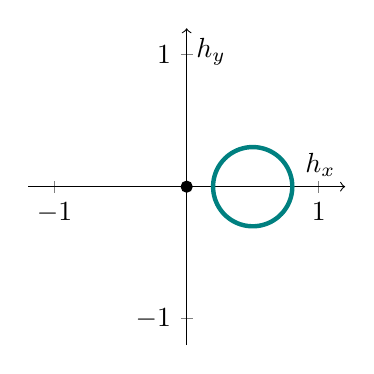
\begin{tikzpicture}
			\begin{axis}[
				axis equal image,
				axis lines=middle,
				axis line style={->},
				xtick={-1,1}, ytick={-1,1},
				xmin=-1.2, xmax=1.2,
				ymin=-1.2, ymax=1.2,
				xlabel=$h_x$, ylabel=$h_y$,
				width=6.5cm,
				]
				\addplot+[mark options={black}] coordinates {(0,0)};
				\addplot [
				samples=100, domain=0:2*pi, color=teal, ultra thick,
				] ( {.3*cos(deg(x)) + .5}, {.3*sin(deg(x))} );
			\end{axis}
		\end{tikzpicture}
		\caption{$v=0.5$, $w=0.3$}
	\end{subfigure}
	\hfil
	\begin{subfigure}{.3\textwidth}
		\centering
		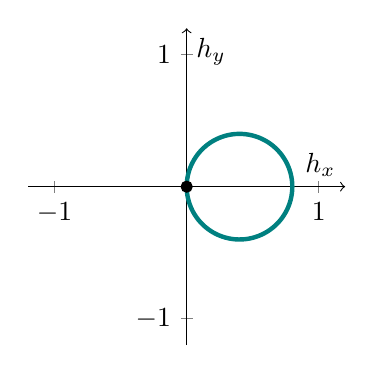
\begin{tikzpicture}
			\begin{axis}[
				axis equal image,
				axis lines=middle,
				axis line style={->},
				xtick={-1,1}, ytick={-1,1},
				xmin=-1.2, xmax=1.2,
				ymin=-1.2, ymax=1.2,
				xlabel=$h_x$, ylabel=$h_y$,
				width=6.5cm,
				]
				\addplot+[mark options={black}] coordinates {(0,0)};
				\addplot [
				samples=100, domain=0:2*pi, color=teal, ultra thick,
				] ( {.4*cos(deg(x)) + 0.4}, {.4*sin(deg(x))} );
			\end{axis}
	\end{tikzpicture}
	\caption{$v=w=0.4$}
	\end{subfigure}
	\hfil
	\begin{subfigure}{.3\textwidth}
		\centering
		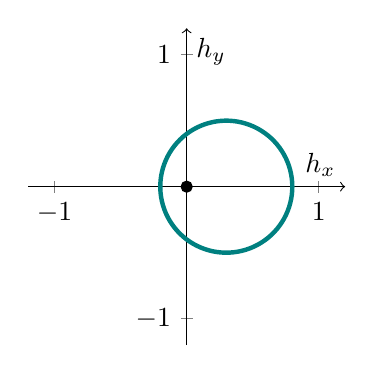
\begin{tikzpicture}
			\begin{axis}[
				axis equal image,
				axis lines=middle,
				axis line style={->},
				xtick={-1,1}, ytick={-1,1},
				xmin=-1.2, xmax=1.2,
				ymin=-1.2, ymax=1.2,
				xlabel=$h_x$, ylabel=$h_y$,
				width=6.5cm,
				]
				\addplot+[mark options={black}] coordinates {(0,0)};
				\addplot [
				samples=100, domain=0:2*pi, color=teal, ultra thick,
				] ( {.5*cos(deg(x)) + 0.3}, {.5*sin(deg(x))} );
			\end{axis}
		\end{tikzpicture}
		\caption{$v=0.3$, $w=0.5$}
	\end{subfigure}
	\caption{Contours in Hamiltonian space for (a) trivial, (b) conducting and (c) topological phases.}
	\label{fig:phases}
\end{figure}

We are now in a position to start analysing the physics of the system. Concretely, the momentum space Hamiltonian is given by
\begin{align*}
	\Hc(k) &= \h(k)\cdot\bm{\upsigma} = \big[v + w\cos(k)\big]\sigma_x + w\sin(k)\sigma_y = \begin{pmatrix}
		0 & v + w\e^{-ik} \\
		v + w\e^{ik} & 0
	\end{pmatrix}.
\end{align*}
We can set up a Fourier transform to real space by rewriting this suggestively in terms of the unit cell index $n$:
\[
	\Hc(k) = \e^{-ik(n-n)}\begin{pmatrix}
		0 & v \\
		v & 0
	\end{pmatrix} + \e^{-ik[(n+1)-n]}\begin{pmatrix}
		0 & w \\
		0 & 0
	\end{pmatrix} + \e^{-ik\big[n-(n+1)\big]}\begin{pmatrix}
		0 & 0 \\
		w & 0
	\end{pmatrix}
\]
The exponentials in this expression are turned into real space delta functions under Fourier transformation, which indicates that the eigenstates are highly confined around certain positions. This is precisely the setting for the tight-binding approximation discussed in Section~\ref{sec:band-theory}. It follows that we can write the Hamiltonian in an exact unit cell basis as
\begin{equation}\label{eq:SSH-n-Hamil}
		\hat{H} = \sum_{n=-\infty}^{\infty}\left[\ket{n}\bra{n}\otimes\begin{pmatrix}
			0 & v \\
			v & 0
		\end{pmatrix} + \left(\ket{n+1}\bra{n}\otimes\begin{pmatrix}
			0 & w \\
			0 & 0
		\end{pmatrix} + {\rm h.c.}\right)\right], 
\end{equation}
where ``h.c.'' denotes the Hermitian conjugate of the preceding term. This Hamiltonian contains a term which acts within the unit cells, and terms which act between neighbouring unit cells, parametrized by $v$ and $w$ respectively. The structure of these interactions can be made somewhat more transparent by going to a finite chain of length $N$. The Hamiltonian then becomes
\[
	\hat{H} = \sum_{n=0}^{N}\ket{n}\bra{n}\otimes\begin{pmatrix}
		0 & v \\
		v & 0
	\end{pmatrix} + \sum_{n=0}^{N-1}\left(\ket{n+1}\bra{n}\otimes\begin{pmatrix}
		0 & w \\
		0 & 0
	\end{pmatrix} + {\rm h.c.}\right),
\]
where open boundary conditions have been introduced on the ends of the chain to allow the boundary behaviour to be studied. The tensor products can be expanded in order to cast the Hamiltonian into a full $2N\times 2N$ matrix:
\[
	\hat{H} = \begin{pNiceMatrix}
		\Block[borders={bottom,right,tikz=dashed}]{2-2}{}
					 0 & v & \Block[borders={bottom,right,tikz=dashed}]{2-2}{}
							 0 & 0 & \Block{4-4}{0} &        &   & \\
					 v & 0 & w & 0 &                &        &   & \\
		\Block[borders={bottom,right,tikz=dashed}]{2-2}{}
					 0 & w & 0 & v &                &        &   & \\
					 0 & 0 & v & 0 &                &        &   & \\
		\Block{4-4}{0} &   &   &   &                & \Ddots & 0 & 0 \\
					   &   &   &   & \Ddots         &        & w & 0 \\
					   &   &   &   &              0 & w      & 0 & v \\
					   &   &   &   &              0 & 0      & v & 0
	\end{pNiceMatrix}.
\]
A physical interpretation of this system presents itself in the form of this matrix: it describes a chain of $2N$ sites, with alternating hopping amplitudes $v$ and $w$ between neighbouring sites. The unit cells now consist of two of these sites, and $v$ and $w$ are referred to as the \emph{intra-cell} and \emph{inter-cell} hoppings, respectively. When these two hoppings are equal, the system is in the gapless phase $v=w$, corresponding to a chain where all bonds are equally strong. Intuitively, this homogeneity allows electrons to propagate freely along the chain. On the other hand, in the insulating cases $v\neq w$, one of the two hoppings is stronger than the other, and the electrons tend to be confined around these stronger bonds.

Dividing the unit cells into two individual sites in this way allows us to distinguish two so-called \emph{sublattices} of the crystal, which we label $A$ and $B$. The notation can then be simplified by labelling quantum states according to the sublattice on which they are localized:
\[
	\ket{n,A} \equiv \ket{n}\otimes\begin{pmatrix}
		1 \\ 0
	\end{pmatrix},\quad \ket{n,B} \equiv \ket{n}\otimes\begin{pmatrix}
		0 \\ 1
	\end{pmatrix}.
\]
In this notation, the Hamiltonian becomes
\begin{equation}\label{eq:ssh-sublattice}
	\hat{H} = \left(\sum_{n=0}^{N}v\ket{n,B}\bra{n,A} + \sum_{n=0}^{N-1}w\ket{n+1,A}\bra{n,B}\right) + {\rm h.c.}
\end{equation}

The tight-binding model of alternating hoppings is precisely the SSH model as it was introduced in 1979 by Wu-Pei Su, John Robert Schrieffer, and Alan J. Heeger \cite{SSH_model,SSH_model2}. It was devised as a model for polyacetylene, a polymer chain which features alternating single and double covalent bonds; see Figure~\ref{fig:polyacetylene}.
\begin{figure}[htb!]
	\centering
	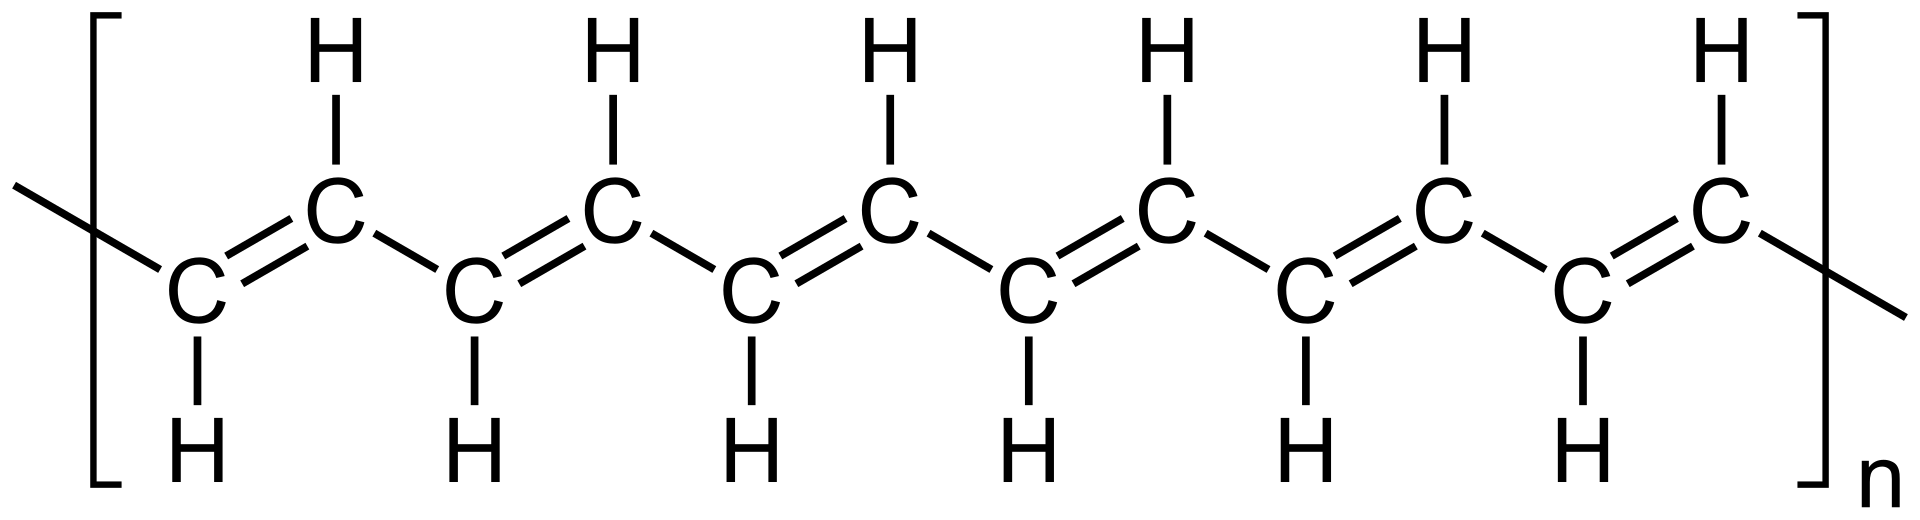
\includegraphics[width=.8\linewidth]{Images/polyacetylene}
	\caption{Structural diagram of polyacetylene. Electrons are transported more readily along the double bonds, which is modelled using a larger hopping parameter.}
	\label{fig:polyacetylene}
\end{figure}
This material displays unexpectedly high conductivity when doped with halogen impurities, and the SSH model affords an explanation for this.

To understand how this metallic behaviour comes about, the differences between the trivial and the topological phase must be examined more closely. The two phases appear to be identical at a first glance: if the unit cell in polyacetylene is chosen in such a way that the stronger double bond represents the intra-cell hopping $v$, then the system is in the trivial phase $v>w$, and if instead the unit cell is centred around a single bond, $v<w$ and the phase is topological. In either case, valence electrons are expected to remain localized around the double bonds, leading to the same insulating bulk behaviour.\footnote{
	The attentive reader might wonder why the conducting $v=w$ phase does not occur naturally in this system. This is a result of the so-called Peierls transition: in a nutshell, introducing a band gap locally lowers the energy of the (filled) valence band and raises that of the (empty) conduction band. This makes it energetically favourable for atoms in the chain to pair up, in a process referred to as dimerisation.}

The difference between the two phases only becomes apparent when the endpoints of the chain are studied. For example, the leftmost atom is not subject to any inter-cell hopping, and it is only connected to the other atom in its unit cell. In the trivial case, this connection is strong and the two atoms share their valence electrons. In the topological phase, on the other hand, the second atom from the left prefers to share electrons with its right-hand neighbour, and the leftmost atom becomes isolated. In the limit where $v$ goes to zero, this isolation becomes complete; this is illustrated in Figure~\ref{fig:SSH-boundaries}.
\begin{figure}[htb!]
	\centering
	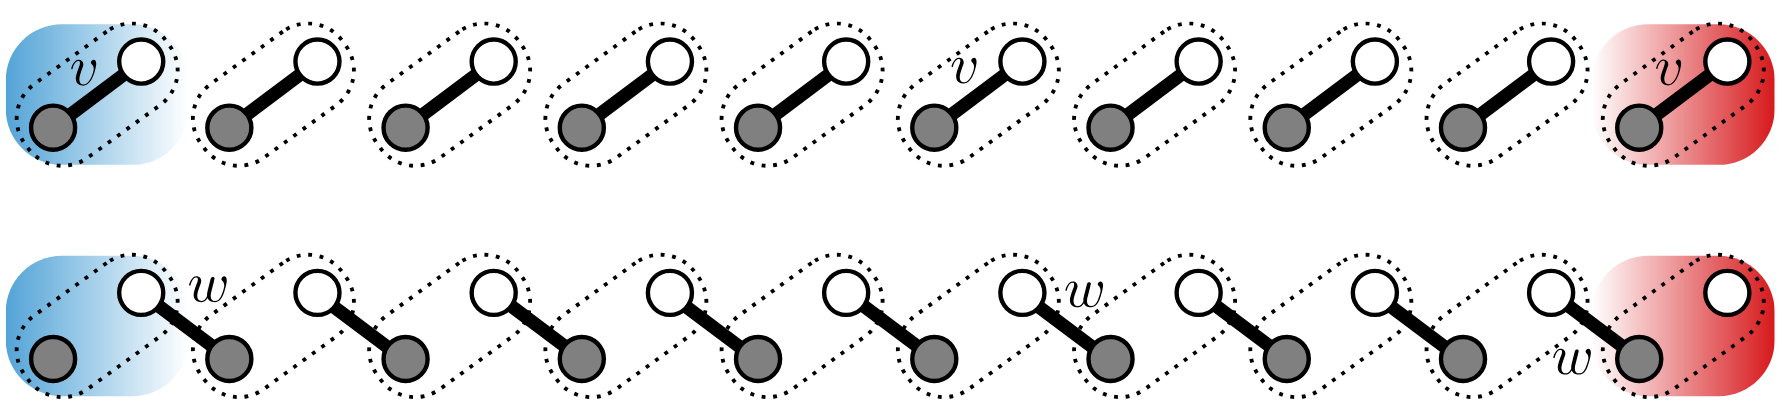
\includegraphics[width=0.8\linewidth]{Images/SSH-boundaries}
	\caption{Figure from Ref.~\cite{Asboth_topo-course}. Top: when $v$ is the dominant hopping term, the boundaries of the chain (indicated in blue and red) do not feature any interesting topology. Bottom: for small enough $v$, there is one atomic site at each boundary that becomes individually isolated from the rest of the chain.}
	\label{fig:SSH-boundaries}
\end{figure}
and the edge sites carry zero-energy eigenstates. In this case, only the second term in the Hamiltonian \eqref{eq:ssh-sublattice} survives, and the edges obey the eigenvalue equations
\begin{align*}
	\hat{H}\ket{1,A} = \hat{H}\ket{N,B} = 0.
\end{align*}
These edge modes can be shown to persist for non-zero $v<w$, in which case they become highly localized and approach zero energy in the $N\to\infty$ limit \cite{Asboth_topo-course}. The salient point is that the boundary modes of the topological phase exist inside the energy gap: their energy eigenvalues have a point-like degeneracy at the Fermi level $E_F = 0$. 

Something remarkable has happened: we have started from a topological description of a gapped bulk phase, and the resulting physical effects appear as in-gap zero energy modes on the boundary of the material. As will become apparent upon looking at other examples, the existence of edge modes at the Fermi level is a fairly general feature of topological phases of matter,\footnote{
	This is not a completely general statement: topological phases with edge modes at energies other than $E_F$ have been shown to be theoretically feasible \cite{Freedman_gapped-edge}. For our purposes, it will be sufficient to restrict our attention to edge modes at the Fermi level.}
captured in the so-called \emph{bulk-boundary correspondence}. It can be thought of as being a result of the inability to go continuously from a topological gapped phase to a trivial one in real space; in particular, the outside boundary of an idealised material connects to the vacuum, which is also considered a trivial gapped phase.

The existence of zero-energy boundary modes is what helps explain the unusual conductivity of doped polyacetlylene. It turns out that introducing impurities promotes the formation of domains with different topological phases within the material. The boundaries between these domains carry charge and their zero energy ensures that they are mobile. As such, they can be described as moving quasiparticle excitations called \emph{solitons}, and the large current response of the material can be attributed to them. These soliton states have since been observed experimentally \cite{Meier_SSH-soliton}, as has the change in Berry phase associated with the topological invariant in Equation~\eqref{eq:SSH-Berry} \cite{Atala_SSH-Zak}.

To close out this section, we return to the physical interpretation of imposing $h_z = 0$, which is the constraint that allowed for non-trivial topology to arise in the first place. This interpretation comes from the fact that the $2\times2$ matrices in the Hamiltonian in Equation~\eqref{eq:SSH-n-Hamil} act between the two different sublattices $A$ and $B$. The exclusion of a $h_z$ term ensures that these matrices only have off-diagonal elements; that is, states can hop from sublattice $A$ to sublattice $B$ and vice versa, but never within either of the two sublattices. This is called \emph{sublattice symmetry} or \emph{chiral symmetry}, and it can be captured in terms of operators. This is done by defining the projection onto either sublattice,
\[
\hat{P}_A = \Id \otimes \begin{pmatrix}
	1 & 0 \\ 0 & 0
\end{pmatrix},\quad \hat{P}_B = \Id \otimes \begin{pmatrix}
	0 & 0 \\ 0 & 1
\end{pmatrix}.
\]
Sublattice symmetry then implies that the Hamiltonian obeys the following relations:
\[
\hat{P}_A\hat{H}\hat{P}_A = \hat{P}_B\hat{H}\hat{P}_B = 0.
\]
Making use of the fact that $\hat{P}_A +\hat{P}_B = \Id$, the chiral symmetry on the Hamiltonian can be expressed in the form
\begin{align*}
	\hat{H} &= (\hat{P}_A + \hat{P}_B)\hat{H}(\hat{P}_A + \hat{P}_B) \\
	&= \hat{P}_A\hat{H}\hat{P}_B + \hat{P}_B\hat{H}\hat{P}_A \\
	&= (\hat{P}_A - \hat{P}_B)\hat{H}(\hat{P}_B - \hat{P}_A) \\
	&=: -\hat{\CHR}\hat{H}\hat{\CHR},
\end{align*}
with $\hat{\CHR}:= \hat{P}_A - \hat{P}_B = \Id\otimes\sigma_z$ having the property that $\hat{\CHR} = \hat{\CHR}^{-1} = \hat{\CHR}\herm$. We can think of this symmetry as an anticommutation relation,
\begin{equation}\label{eq:chiral-operator}
	\{\hat{H},\hat{\CHR}\} = 0.
\end{equation}
A similar statement holds in momentum space, where $\sigma_z$ plays the role of $\hat{\CHR}$: there, chiral symmetry can be expressed as
\begin{equation}\label{eq:chiral-momentum}
	\Hc(k) = -\sigma_z\Hc(k)\sigma_z \quad\iff\quad \{\Hc(k),\sigma_z\} = 0,
\end{equation}
which is precisely the case when the Hamiltonian only has $\sigma_x$ and $\sigma_y$ terms.

An immediate consequence of this setup is that the trivial and topological phase become adiabatically connected if we allow for sublattice symmetry breaking ($h_z \neq 0$). This means that the topological phases of the system are dependent on the symmetry remaining unbroken, and as such they are considered to be \emph{protected} by it.


\markedsection{Tenfold way}{The tenfold way of topological matter}\label{sec:symm-classes}

The SSH model discussed in the previous section demonstrates that the topological nature of a system is inextricably linked to the symmetries that it possesses. It should come as no surprise, then, that this relation between topology and symmetry has comprised one of the principal avenues of research in topological matter. In this section, we review one of the most important results of this endeavour, which comes in the form of a periodic table of gapped topological phases of matter---often referred to as the \emph{tenfold way}. Much of the discussion here is borrowed from the review in Ref.~\cite{Ludwig_tenfold-way}.

The idea at the heart of the tenfold way classification is that any symmetry on a quantum mechanical system---not only a crystalline one---can be reduced to several fundamental components. This idea was first developed by Martin Zirnbauer and Alexander Altland around the turn of the current century \cite{Zirnbauer_random-matrix,AltlandZirnbauer_symm-classes,Heinzner_symm-classes}. We summarize the main ideas of the construction here.

First, the system may be subject to a number of ordinary unitary symmetries, such as rotations, reflections, or the spatial translations that define a crystal. Each of these unitary symmetries is represented by a unitary operator $\hat{U}$ that commutes with the Hamiltonian: that is, the symmetry is defined as
\begin{equation*}
	\hat{H} = \hat{U}\hat{H}\hat{U}^{-1}.
\end{equation*}
It turns out that one can always find a basis for the Hilbert space in which the Hamiltonian is block diagonal, with none of the blocks commuting with any unitary operator individually. As a consequence, the structure of any Hamiltonian can in principle be understood by considering only the symmetries which are not of this form.

Remarkably, it transpires that there are only three basic operations which generate the remainder of the possible symmetries.
The first of these three is the chiral or sublattice symmetry $\hat{\CHR}$ that we have already encountered in the context of the SSH model. As seen in Equations~\eqref{eq:chiral-operator} and \eqref{eq:chiral-momentum}, the chiral symmetry operator is unitary, but it anti-commutes with the Hamiltonian.

The second remaining type of symmetry is time-reversal invariance. It is generated by an anti-unitary operator $\hat{\TRS}$ that commutes with the Hamiltonian,
\begin{equation*}
	\hat{H} = \hat{\TRS}\hat{H}\hat{\TRS}^{-1}.
\end{equation*}
Anti-unitarity implies that $\hat{\TRS}$ combines a unitary transformation with complex conjugation. This can be seen to hold for time reversal by noting that the reflection $t\mapsto -t$ acts on the time evolution operator $\e^{i\hat{H}t}$ as complex conjugation. 

Importantly, it can be shown that the time reversal operator $\hat{\TRS}$ must square to $\hat{\TRS}^2=\pm\Id$, with the positive and negative signs corresponding to bosonic and fermionic statistics, respectively. In momentum space, time-reversal symmetry can be written as
\begin{equation*}
	\Hc(\k) = U\Hc^*(-\k)U^{-1},
\end{equation*}
where $U$ is a unitary matrix and the momentum vector $\k$ may have any number of dimensions. The sign change in $\k$ is due to the fact that momentum has a time component.

The final possible symmetry of the system is that of charge conjugation, also known as particle-hole symmetry. It is associated with an anti-unitary operator $\hat{\PHS}$ that anti-commutes with the Hamiltonian:
\begin{equation*}
	\hat{H} = -\hat{\PHS}\hat{H}\hat{\PHS}^{-1}.
\end{equation*}
Just like the time-reversal operator, $\hat{\PHS}$ can square to two different values $\hat{\PHS}^2 = \pm\Id$, yielding physically inequivalent systems.

These three basic symmetry operations are subject to the relation
\begin{equation*}
	\hat{\CHR} = \hat{\TRS}\hat{\PHS},
\end{equation*}
which implies that a system satisfying any two of the symmetries automatically satisfies the third as well. As a result, there are a total of ten distinct ways of combining the three symmetries, each giving rise to a so-called \emph{symmetry class}. These ten symmetry classes are exactly what makes up the titular \emph{tenfold way}, and they are listed on the left hand side of Table~\ref{tbl:tenfold-way}.\footnote{
	While the names of the classes are seemingly disordered, they are borrowed from mathematician Élie Cartan's 1926 classification of a subtly related set of geometric spaces.}
\begin{table}[htb!]
\centering
\setlength{\tabcolsep}{8pt}
\renewcommand{\arraystretch}{1.2}
\begin{NiceTabular}{l|ccc!{\ }||ccccccccc}
	\CodeBefore
		\rowcolors{2}{gray!10}{white}[cols=2-*]
	\Body
	\Hline[tikz={line width=1.2pt}]
	\multicolumn{4}{c|}{\textbf{Symmetry\ }} & \multicolumn{9}{c}{\textbf{Dimension}} \\
	\Hline
	\textbf{Class} & $\mathbf{\TRS^2}$ & $\mathbf{\PHS^2}$ & $\mathbf{\CHR}$ & 
	$\mathbf{0}$ & $\mathbf{1}$ & $\mathbf{2}$ & $\mathbf{3}$ & 
	$\mathbf{4}$ & $\mathbf{5}$ & $\mathbf{6}$ & $\mathbf{7}$ & $\mathbf{8}$ \\
	\Hline
	A     & 0  & 0  & 0 & $\Z$   & 0      & $\Z$   & 0      & $\Z$   & 0      & $\Z$   & 0      & $\Z$   \\
	AIII  & 0  & 0  & 1 & 0      & $\Z$   & 0      & $\Z$   & 0      & $\Z$   & 0      & $\Z$   & 0      \\
	\Hline[color=gray!75,tikz=densely dashed] 
	AI    & +1 & 0  & 0 & $\Z$   & 0      & 0      & 0      & $2\Z$  & 0      & $\Z_2$ & $\Z_2$ & $\Z$   \\
	BDI   & +1 & +1 & 1 & $\Z_2$ & $\Z$   & 0      & 0      & 0      & $2\Z$  & 0      & $\Z_2$ & $\Z_2$ \\
	D     & 0  & +1 & 0 & $\Z_2$ & $\Z_2$ & $\Z$   & 0      & 0      & 0      & $2\Z$  & 0      & $\Z_2$ \\
	DIII  & –1 & +1 & 1 & 0      & $\Z_2$ & $\Z_2$ & $\Z$   & 0      & 0      & 0      & $2\Z$  & 0      \\
	AII   & –1 & 0  & 0 & $2\Z$  & 0      & $\Z_2$ & $\Z_2$ & $\Z$   & 0      & 0      & 0      & $2\Z$  \\
	CII   & –1 & –1 & 1 & 0      & $2\Z$  & 0      & $\Z_2$ & $\Z_2$ & $\Z$   & 0      & 0      & 0      \\
	C     & 0  & –1 & 0 & 0      & 0      & $2\Z$  & 0      & $\Z_2$ & $\Z_2$ & $\Z$   & 0      & 0      \\
	CI    & +1 & –1 & 1 & 0      & 0      & 0      & $2\Z$  & 0      & $\Z_2$ & $\Z_2$ & $\Z$   & 0      \\
	\Hline[tikz={line width=1.2pt}]
\end{NiceTabular}
\caption{Tenfold classification of gapped topological states. The names of all ten symmetry classes are listed on the left, together with the choices of symmetries that they represent---in particular, the columns corresponding to $\hat{\TRS}$ and $\hat{\PHS}$ also list the sign of the squared operator. The dashed horizontal line separates the two complex symmetry classes above from the eight real ones below. The right hand side lists all possible topological invariants in each symmetry class in various dimensions, under the assumption of no commuting unitary symmetries. The table of invariants shows Bott periodicity in the number of dimensions: the complex classes repeat after two columns, and the real classes repeat after eight.}
\label{tbl:tenfold-way}
\end{table}

The ten different symmetry classes appearing in this scheme each pose their own unique constraints on the Hamiltonians that are allowed in a system. Importantly, these constraints affect the topology of the abstract space of permissible non-zero Hamiltonians, allowing for the existence of different non-trivial gapless phases. The precise classification of all these phases is rather involved, and for our purposes we will settle for presenting its results on the right hand side of Table~\ref{tbl:tenfold-way}. Still, we have already seen a simple example of these principles play out in the case of the SSH model in Section~\ref{sec:SSH}: there, imposing chiral symmetry transformed the Hamiltonian space from $\R^3\setminus\set{0}$ to $\R^2\setminus\set{0}$, allowing the one-dimensional Brillouin zone $S^1$ to map into it with a non-trivial $\Z$-valued winding number. This is reflected exactly in the table of invariants: imposing chiral symmetry takes us from class A to AIII, and in one dimension this changes the invariant group from a trivial $0$ to $\Z$.

One striking feature of this table of invariants is that it is a periodic table, in the most literal sense. That is, there is a repeating pattern in the table across eight dimensions. More specifically, the symmetry classes are divided up into two \emph{complex} classes and eight \emph{real} classes---the latter being so called because the anti-unitary symmetries act similarly to the reality condition $\hat{H} = \hat{H}*$. There is then a mod 2 periodicity in the complex classes and a mod 8 periodicity in the real classes. These repetitions turn out to be directly related to a deep mathematical result called Bott periodicity. This result manifests itself in different ways across homotopy, K-theory and the theory of Clifford algebras. For example, the generalised cohomology groups in $K$ theory have a mod 2 periodicity, and their real $KO$ counterparts repeat mod 8. Unfortunately, there is no direct analogue of this result in our preferred standard cohomology setting, and we will not pay it too much mind.

The full tenfold way classification of topological invariants has been of immense importance in the study of topological matter, and doubtless many condensed matter physicists have a variation of Table~\ref{tbl:tenfold-way} affixed to their fridge door. For any given system in any number of dimensions, it immediately informs of the topological phases that can be expected, as long as the basic symmetries are known. Still, there are some important caveats to the interpretation of this table; before we move on to more examples of specific systems, we cover two limitations that are of importance in our own research.

First, this classification scheme assumes a general $N$-band description. While many of the invariants listed in this table can be obtained equally well in our simplified two-band model of choice, this does not hold across the board. For example, the $\Z$ invariant for a zero-dimensional class A Hamiltonian (i.e.\ a generic Hermitian matrix) can be interpreted as the number of occupied bands in the system (i.e.\ the number of negative eigenvalues). In any given scenario, this may reflect both positively and negatively on the usefulness of the two-band model: on the one hand, it can indicate that the two bands do not carry enough degrees of freedom for a full description. On the other hand, topological invariants which are not stable under the addition of bands away from the Fermi level may not be indicative of any transport phenomena, and these may get ``filtered out'' in the two-band description---we demonstrate a tentative example of this in our treatment of inversion-symmetric Weyl semimetals in Section~\ref{sec:inversion-existing}.

Second, note that this table specifically records only the invariants which are not protected by a commutative unitary symmetry. Such invariants are called \emph{strong} in the sense that they do not rely on any assumption of translation or similar symmetries. Nevertheless, in a regular crystalline solid, the translation symmetries routinely give rise to additional \emph{weak} invariants, relating to lower-dimensional entries on the table. We will study three-dimensional examples of this in class AII and A, in Sections~\ref{sec:3D-Z2} and \ref{sec:3D-Chern} respectively. Besides translation, the real-space lattice may also be subject to other symmetries such as rotations and reflections. A comprehensive account of the topological effects of these symmetries in three dimensions is given in Ref.~\cite{Shiozaki_AHSS}.


\markedsection{2D and 3D examples}{Higher-dimensional examples}\label{sec:insulators}

With the tenfold way in hand, we are now in a good position to review some additional examples of non-trivial topological materials. We will be very brief in our treatment of these systems, and approach them from a generic topological point of view. Readers wishing to learn more about the properties of their physical realisations are referred to the more comprehensive physics-minded overviews in standard references such as Refs.~\cite{Bernevig_topological-insulators,Asboth_topo-course,Akhmerov_online-course}.

\subsection{The Chern insulator}\label{sec:Chern}

A very important class of topological insulators are the so-called \emph{Chern insulators}. These are two-dimensional systems with no additional symmetries beyond lattice translation, i.e.\ in symmetry class A of the tenfold way. In Table~\ref{tbl:tenfold-way}, it is shown that such two-dimensional class A systems have an integer invariant associated with them.

The invariant on these systems is a so-called \emph{Chern number}, and it can be expressed in terms of the total curvature of the Berry connection:
\begin{equation}\label{eq:Chern-number}
	C = \frac{1}{2\pi}\int_{\T^2} \Fc,
\end{equation}
where $\T^2$ is the two-dimensional Brillouin torus and $\Fc$ is the Berry curvature 2-form as defined in Section~\ref{sec:band-theory}. This total curvature represents the $\U(1)$ phase change picked up by a state after parallel transport around the full $\T^2$, and as such it must be quantized to a multiple of $2\pi$.

The Chern number essentially classifies the curvature 2-form $\Fc$ into different cohomology classes on the Brillouin torus, as outlined in Section~\ref{sec:cohomology}. That is, we can consider $\Fc$ to be a representative of the second cohomology class\footnote{
	As explained in Section~\ref{sec:cohomology}, $\Fc$ more properly represents a class in the real-valued de Rham cohomology group $H_{\rm dR}^2(\T^2)\cong\R$. The analogy is strong enough to be considered direct here, but de Rham cohomology is too plain to encode features such as $\Z_2$ invariants. This is why we make use of the richer integer-valued cohomology theory throughout this work.}
\begin{equation*}
	[\Fc] \in H^2(\T^2) \cong \Z.
\end{equation*}
The Chern number can then be thought of as an element of this integer group $\Z$. This means that the cohomology group $H^2(\T^2)$ precisely classifies the different topological phases of a Chern insulator.\footnote{
	More fundamentally, a complex line bundle called the \emph{valence bundle} can be associated to a gapped Hamiltonian, and the second cohomology group (i.e.\ the Chern number) classifies the different complex line bundles over a manifold---it is an example of a so-called \emph{characteristic class}. The vector bundle classification point of view is not one we will pursue in detail in this work, but it is in some ways more fundamental than the description in terms of Berry curvature, especially for systems with additional symmetries. This makes it the preferred point of view for precise mathematical classification schemes---often in the form of K-theory.}

Physically, the best-known realisation of the Chern insulator comes in the form of the \emph{quantum Hall effect}, whereby a magnetic field induces a directional current in the edge of a two-dimensional material. Under the right conditions, this current is quantised, leading to discrete plateaus in the Hall conductance of the material \cite{vKDP_QHE,vonKlitzing_QHE}. This effect was found to be described by a Chern number \cite{TKNN}. The discovery of the quantum Hall effect in 1980 and its subsequent description in terms of a topological invariant in 1982 can be considered formative events in the field of topological matter, and both have been rewarded with a Nobel Prize in Physics \cite{Nobel_1985,Nobel_2016}.

The conducting edge state that appears in the quantum Hall effect is a manifestation of the bulk-boundary correspondence that was introduced in Section~\ref{sec:SSH} in the context of the SSH model. It is the result of the fact that the edge forms a boundary between the topological quantum Hall state and the vacuum, which is a trivial insulator. In terms of dispersion, this edge mode presents itself as a directional band crossing between the valence and conduction bands, on the one-dimensional Brillouin zone of the material boundary; see Figure~\ref{fig:QHE_edge-state}.
\begin{figure}[htb!]
	\centering
	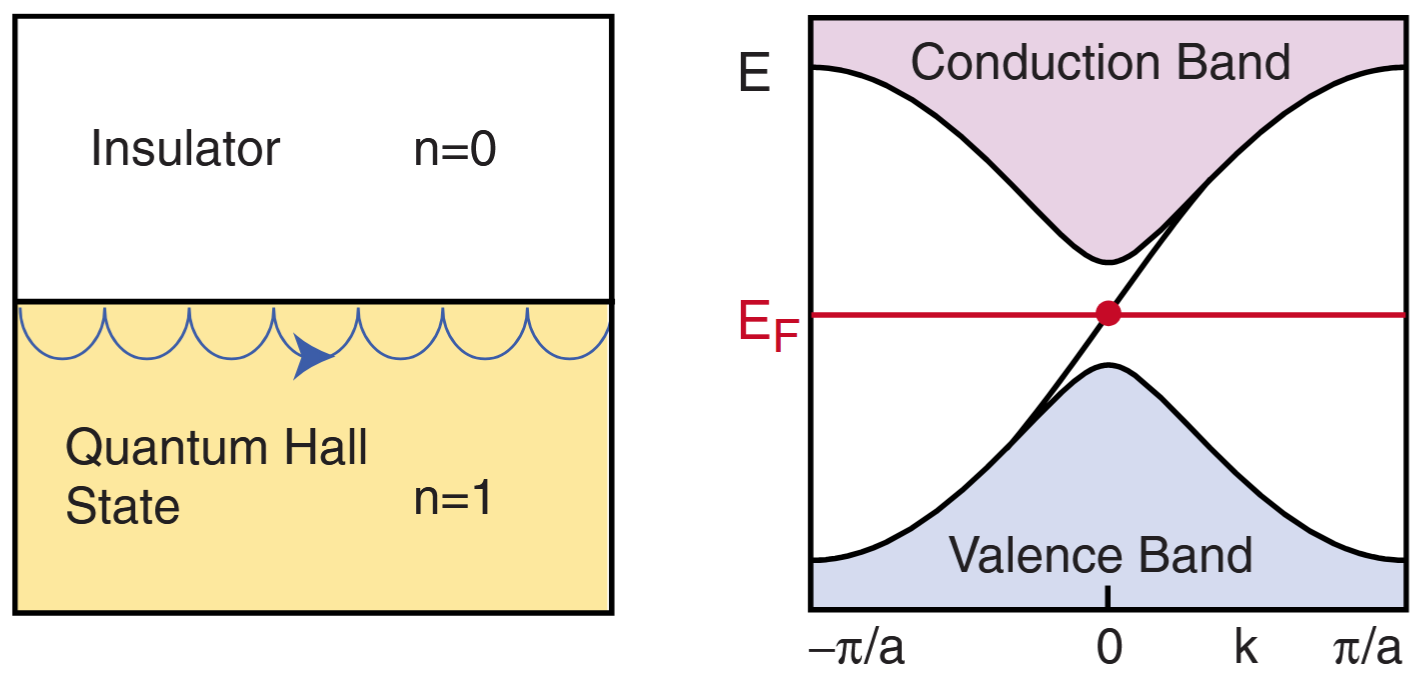
\includegraphics[width=.75\linewidth]{Images/QHE_edge-state}
	\caption{Figure from \cite{HasanKane_colloquium}. Left: The edge current in a quantum Hall state exists on the interface between a topological and a trivial insulator (i.e.\ the vacuum). Right: The conducting edge state corresponds to a chiral band crossing on the one-dimensional surface Brillouin zone, whose chirality is tied to the direction of the current.}
	\label{fig:QHE_edge-state}
\end{figure}
The direction of this band crossing is a chiral feature, and it is directly related to the sign of the Chern number.

For completeness we should make mention of the quantum \emph{anomalous} Hall effect here, which is a related realisation of the Chern insulator that does not depend on an external magnetic field \cite{Haldane_QAHE}. This system is equally well described with a Chern number.


\subsection{Quantum spin Hall effect}\label{sec:QSHE}

Another significant class of topological insulators is that of (fermionic) time-reversal symmetric systems in two dimensions. Table~\ref{tbl:tenfold-way} shows that these class AII systems have a $\Z_2$ invariant associated with them; that is, they are either trivial or topological, with no distinction between different topological phases.

This symmetry class is realised in the \emph{quantum spin Hall effect}, a variant of the quantum Hall effect which was first introduced to describe properties of graphene \cite{KaneMele_QSHE}. This description essentially consists of two copies of the quantum \emph{anomalous} Hall effect described above, one with spin up states and another with spin down states. These copies are given opposite Chern numbers $C_\uparrow = -C_\downarrow$, so that the related edge currents run in opposite directions; see Figure~\ref{fig:QSHE_edge-state}.
\begin{figure}[htb!]
	\centering
	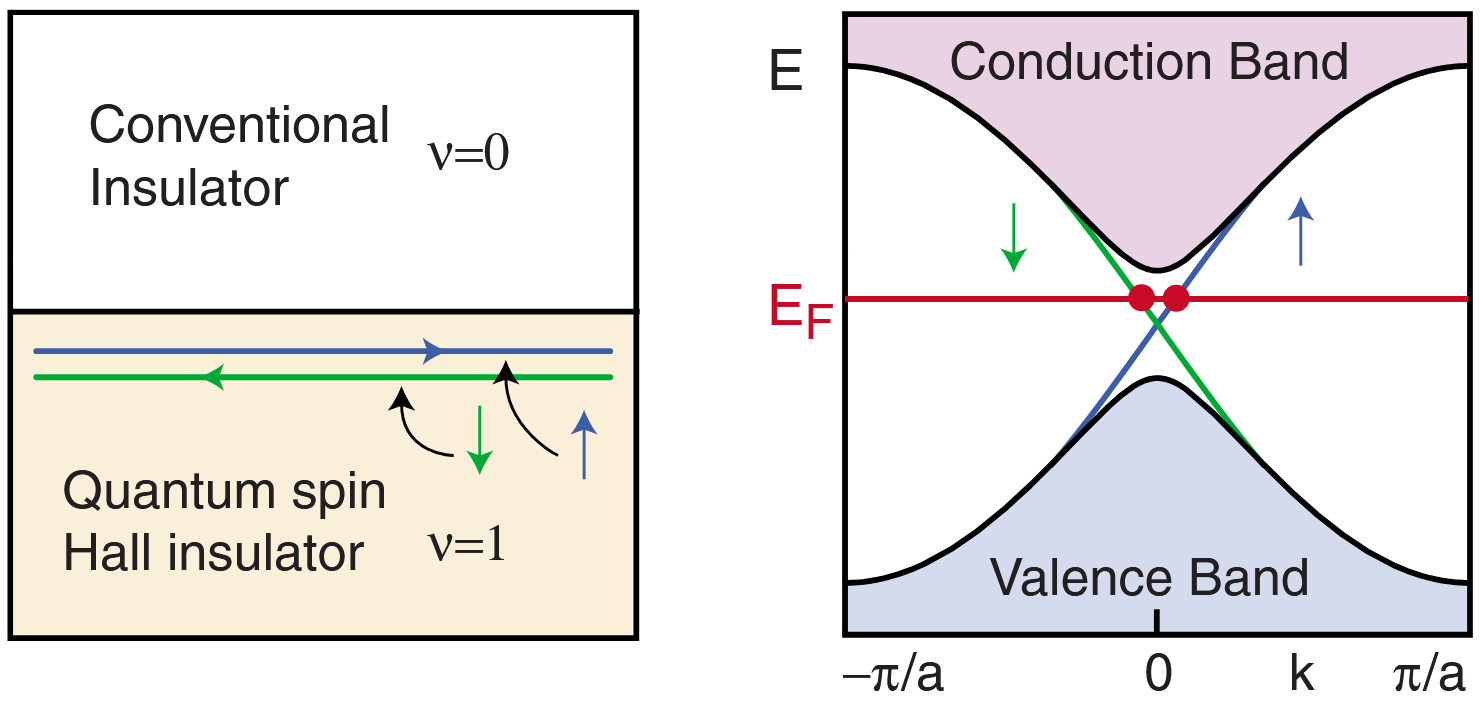
\includegraphics[width=.75\linewidth]{Images/QSHE_edge-state}
	\caption{Figure from \cite{HasanKane_colloquium}. Left: Two edge currents are shown on a quantum spin Hall state: a current of spin up particles running in one direction, and a spin down current in the opposite direction.
		Right: The two opposing edge currents give rise to band crossings of opposite chirality.}
	\label{fig:QSHE_edge-state}
\end{figure}

Because the quantum spin Hall state includes two spin sectors of opposite Chern number, the total Chern number of the system is always zero; as such, it cannot be used to study the topology of such materials. The individual Chern numbers $C_\uparrow$ and $C_\downarrow$ do contain topological information about the system, but they are subject to additional physicality constraints, as reviewed in Ref.~\cite{Sato_superconductors}. There are multiple equivalent ways to define the $\Z_2$ invariant on this system \cite{KaneMele_QSHE-Z2,Sheng_QSHE,MooreBalents_TRS,QHZ_QSHE}. We will not review these in detail here; we only note that there are subtle ties to cohomology, made precise in Ref.~\cite{NittisGomi_FKMM}. This cohomology description also applies to the systems discussed in the next section, and we will postpone our review of it until Section~\ref{sec:T-WSMs}, where it appears in the context of Weyl semimetals.


\subsection{3D strong and weak insulators}\label{sec:3D-Z2}

The final class of insulators we will consider here is that of the three-dimensional time-reversal invariant systems. These are a higher-dimensional extension of the quantum spin Hall states discussed above, and their (3D class AII) entry in Table~\ref{tbl:tenfold-way} suggests that they are subject to a single $\Z_2$ invariant. However, this does not paint the complete picture. As discussed at the end of Section~\ref{sec:symm-classes}, the translation symmetry of the lattice may induce invariants beyond those recorded in Table~\ref{tbl:tenfold-way}. This is also the case here: there are three additional $\Z_2$ invariants related to two-dimensional subspaces of the Brillouin zone \cite{MooreBalents_TRS}.

The idea is as follows. Within the three-dimensional Brillouin zone $\T^3$, there are six special planes which respect time-reversal symmetry; see Figure~\ref{fig:TRIM_3D}.
\begin{figure}[htb!]
	\centering
	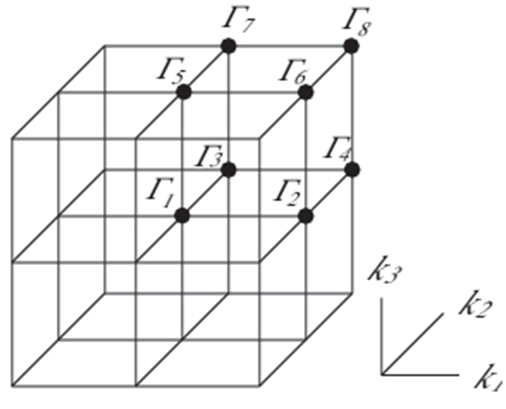
\includegraphics[width=.5\linewidth]{Images/TRIM_3D}
	\caption{Figure from Ref.~\cite{Sato_superconductors}. The three-dimensional Brillouin zone features eight time-reversal invariant momenta (denoted $\Gamma_i$), which satisfy $\k\sim-\k$. Six planes run through these momenta perpendicular to the coordinate directions, and these planes respect time-reversal symmetry as a whole.}
	\label{fig:TRIM_3D}
\end{figure}
Each of these planes has $\T^2$ topology, and so it is equivalent to the Brillouin zone of a two-dimensional quantum spin Hall system. As such, all six feature a $\Z_2$ invariant. The three planes running through the origin define the three weak $\Z_2$ invariants of the system. The topology of the remaining three planes turns out to be fixed by the single strong $\Z_2$ invariant predicted by Table~\ref{tbl:tenfold-way}. When this strong invariant is trivial, parallel planes host the same $\Z_2$ invariant and the system is called a \emph{weak insulator}; conversely, a non-trivial strong invariant gives rise to opposite $\Z_2$ invariants on parallel planes, in what is called a \emph{strong insulator}.

Just as in the two-dimensional case, these systems have a cohomology description which is laid out in Refs.~\cite{NittisGomi_FKMM,BunkSzabo_TRS}; again, we will review aspects of this description in the semimetallic context of the next chapter.